\documentclass{atistandalonetask}
\usepackage{atistandard}

\begin{document}
  \begin{atiTask}[
    title = Integrale mit Delta-Distributionen II
  ]
	Berechnen Sie die Integrale:

    \begin{atiSubequations}
    	\begin{multicols}{2}
    	\item{\integral{-\infty}{\infty}{f(x)\delta(-ax+b)}{x}}
    	\item{\integral{0}{\infty}{\ln x \delta(x^2-1)}{x}}
    	\item{\integral{-\pi}{\pi}{(x+1)^2\delta(\sin \pi x)}{x}}
    	\item{\integral{-\infty}{\infty}{\cos x\delta(x^2-\pi^2)}{x}}
    	\item{\integral{-\infty}{\infty}{f(x)\delta(e^x-1)}{x}}
    	\item{\integral{-\infty}{\infty}{f(x)\delta(x^2+a^2)}{x}\quad a\in \mathbb{R}},
   \end{multicols}	
   \end{atiSubequations}
  \end{atiTask}
  \begin{atiSolution}
   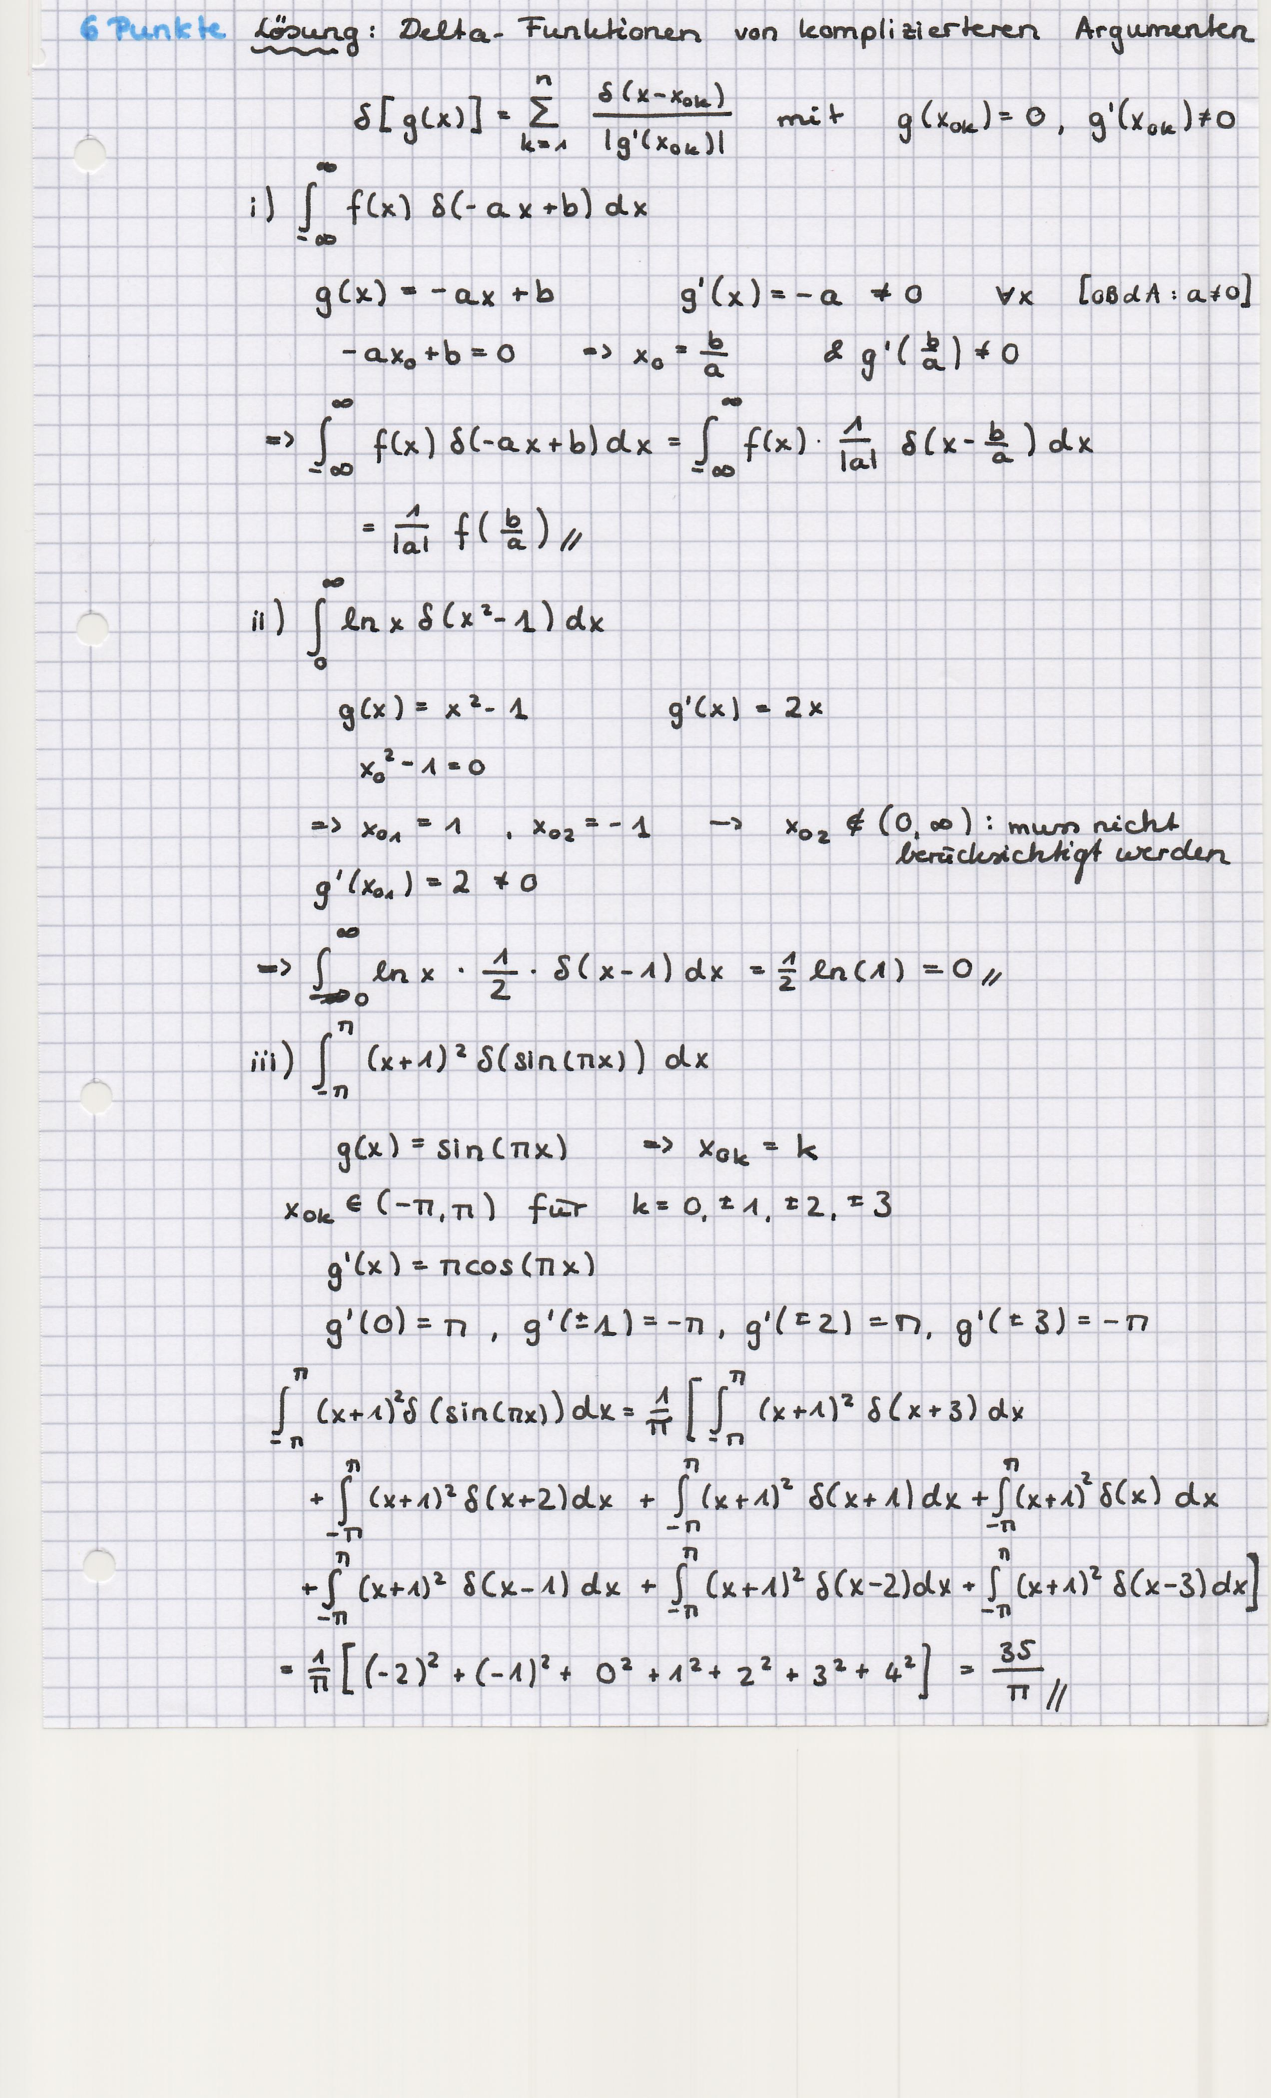
\includepdf[pages=-]{solution-delta_iii.pdf}
  \end{atiSolution}
\end{document}